\section{Introduction}
Acoustic scattering is the physical phenomena of how sound interacts with objects and medium fluctuations. When an acoustic wave hits a rigid object, it is totally reflected, and the object is left in a quiescent state. In the case of an elastic object, part of the sound is transmitted into the object, which is set into motion and starts radiating sound. This leads to a coupled acoustic-structure interaction (ASI) problem.
Applications include underwater acoustics~\cite{Gilroy2013bib} and noise propagation in air~\cite{Bouillard1999eea}. Inverse problems are also of interest, such as shape optimization of membranes~\cite{Manh2011iso} and the problem of designing submarines with low scattering strength. Assuming harmonic time dependency, the fluid and solid media can be modeled using the scalar and vector Helmholtz equations, respectively. The vector Helmholtz equation can be used to model electromagnetic waves~\cite{Manh2012iaa}, such that the work presented herein can also be used for electromagnetic scattering.

Herein, the acoustic scattering characterized by sound waves reflected by man-made elastic objects will be addressed. Shape optimization for optimal acoustic scattering on man-made objects, e.g. antennas, submarines etc., is a typical problem facing design engineers.

Isogeometric analysis (IGA) is basically an extension of the finite element method (FEM) using non-uniform rational B-splines (NURBS) as basis functions not only representing the solution space, but also the geometry. Being introduced in 2005 by Hughes et al.~\cite{Hughes2005iac}, followed by the book~\cite{Cottrell2009iat} in 2009, IGA tries to bridge the gap between finite element analysis (FEA) and computer aided design (CAD) tools. The important feature of IGA is that it uses the same basis as CAD software for describing the given geometry, and thus exact representation of the model is possible.

\begin{figure}
	\centering
	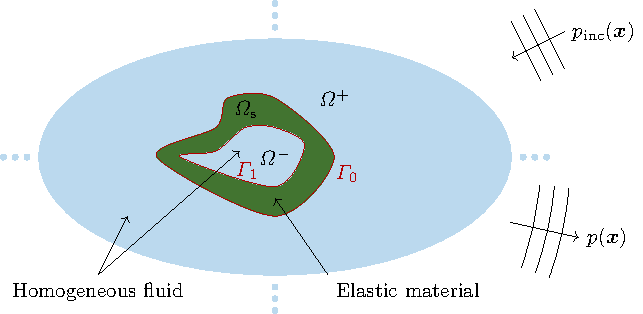
\includegraphics[scale=1]{../../LaTeX/createFigures/TikzFigures/articleIGA_PhD/physicalProblem}
%	\includegraphics[scale=1]{\graphicsFolder/Figure1}
	\caption[Illustration of the physical problem]{Illustration of the physical problem. A plane incident wave, $p_{\mathrm{inc}}(\vec{x})$, is scattered by the scatterer, $\Omega_{\mathrm{s}}$, in an unbounded domain, $\Omega^+$, resulting in the scattered wave, $p(\vec{x})$. The scatterer, which is bounded by the boundaries $\Gamma_0$ and $\Gamma_1$, envelops a fluid domain, $\Omega^-$.}
	\label{Fig2:physicalProblem}
\end{figure}
The physical problem is illustrated in \Cref{Fig2:physicalProblem} where the incoming sound waves, $p_{\rm inc}$, originate from a point source far from this object, such that the (spherical) sound waves are quite accurately approximated by plane waves when the waves reaches the proximity of the object. For rigid objects of irregular shape, the incoming wave may be reflected multiple times before leaving the object. When the object is elastic a coupled ASI problem results. The goal is then to calculate the scattered wave $p$ at an arbitrary far field point. Finally, to use the FEM or IGA the domain must be finite. A fictitious boundary is thus introduced, which must be implemented in such a way that outgoing waves reaching this boundary are absorbed.


The problem at hand is time dependent. However, harmonic time dependency will be assumed, such that all time dependent functions may be written as ${\breve{F}=\breve{F}(\vec{x},t) = F(\vec{x})\euler^{-\imag\omega t}}$ where $\omega$ is the angular frequency and $\imag = \sqrt{-1}$ the imaginary unit. This enables us to model the pressure $p$ in the fluid with the Helmholtz equation given by
\begin{equation}\label{Eq2:HelmholtzEquationIntro}
	\nabla^2 p + k^2 p = 0
\end{equation}
with the wave number $k=\frac{\omega}{c_{\mathrm{f}}}$ (where $c_{\mathrm{f}}$ is the wave speed in the fluid). Other important quantities include the frequency $f=\frac{\omega}{2\PI}$ and the wavelength $\lambda = \frac{2\PI}{k}$.

The geometry of the elastic object may be quite complex but is typically exactly represented using NURBS. This fact is one of the motivating factors for using IGA, as it uses the same functions as basis functions for analysis. The spherical shell depicted in \Cref{Fig2:SphericalShell} is an example of a geometry that has an exact representation using NURBS but is outside the space of standard (Lagrangian) FEM geometries.
\begin{figure}
	\centering
	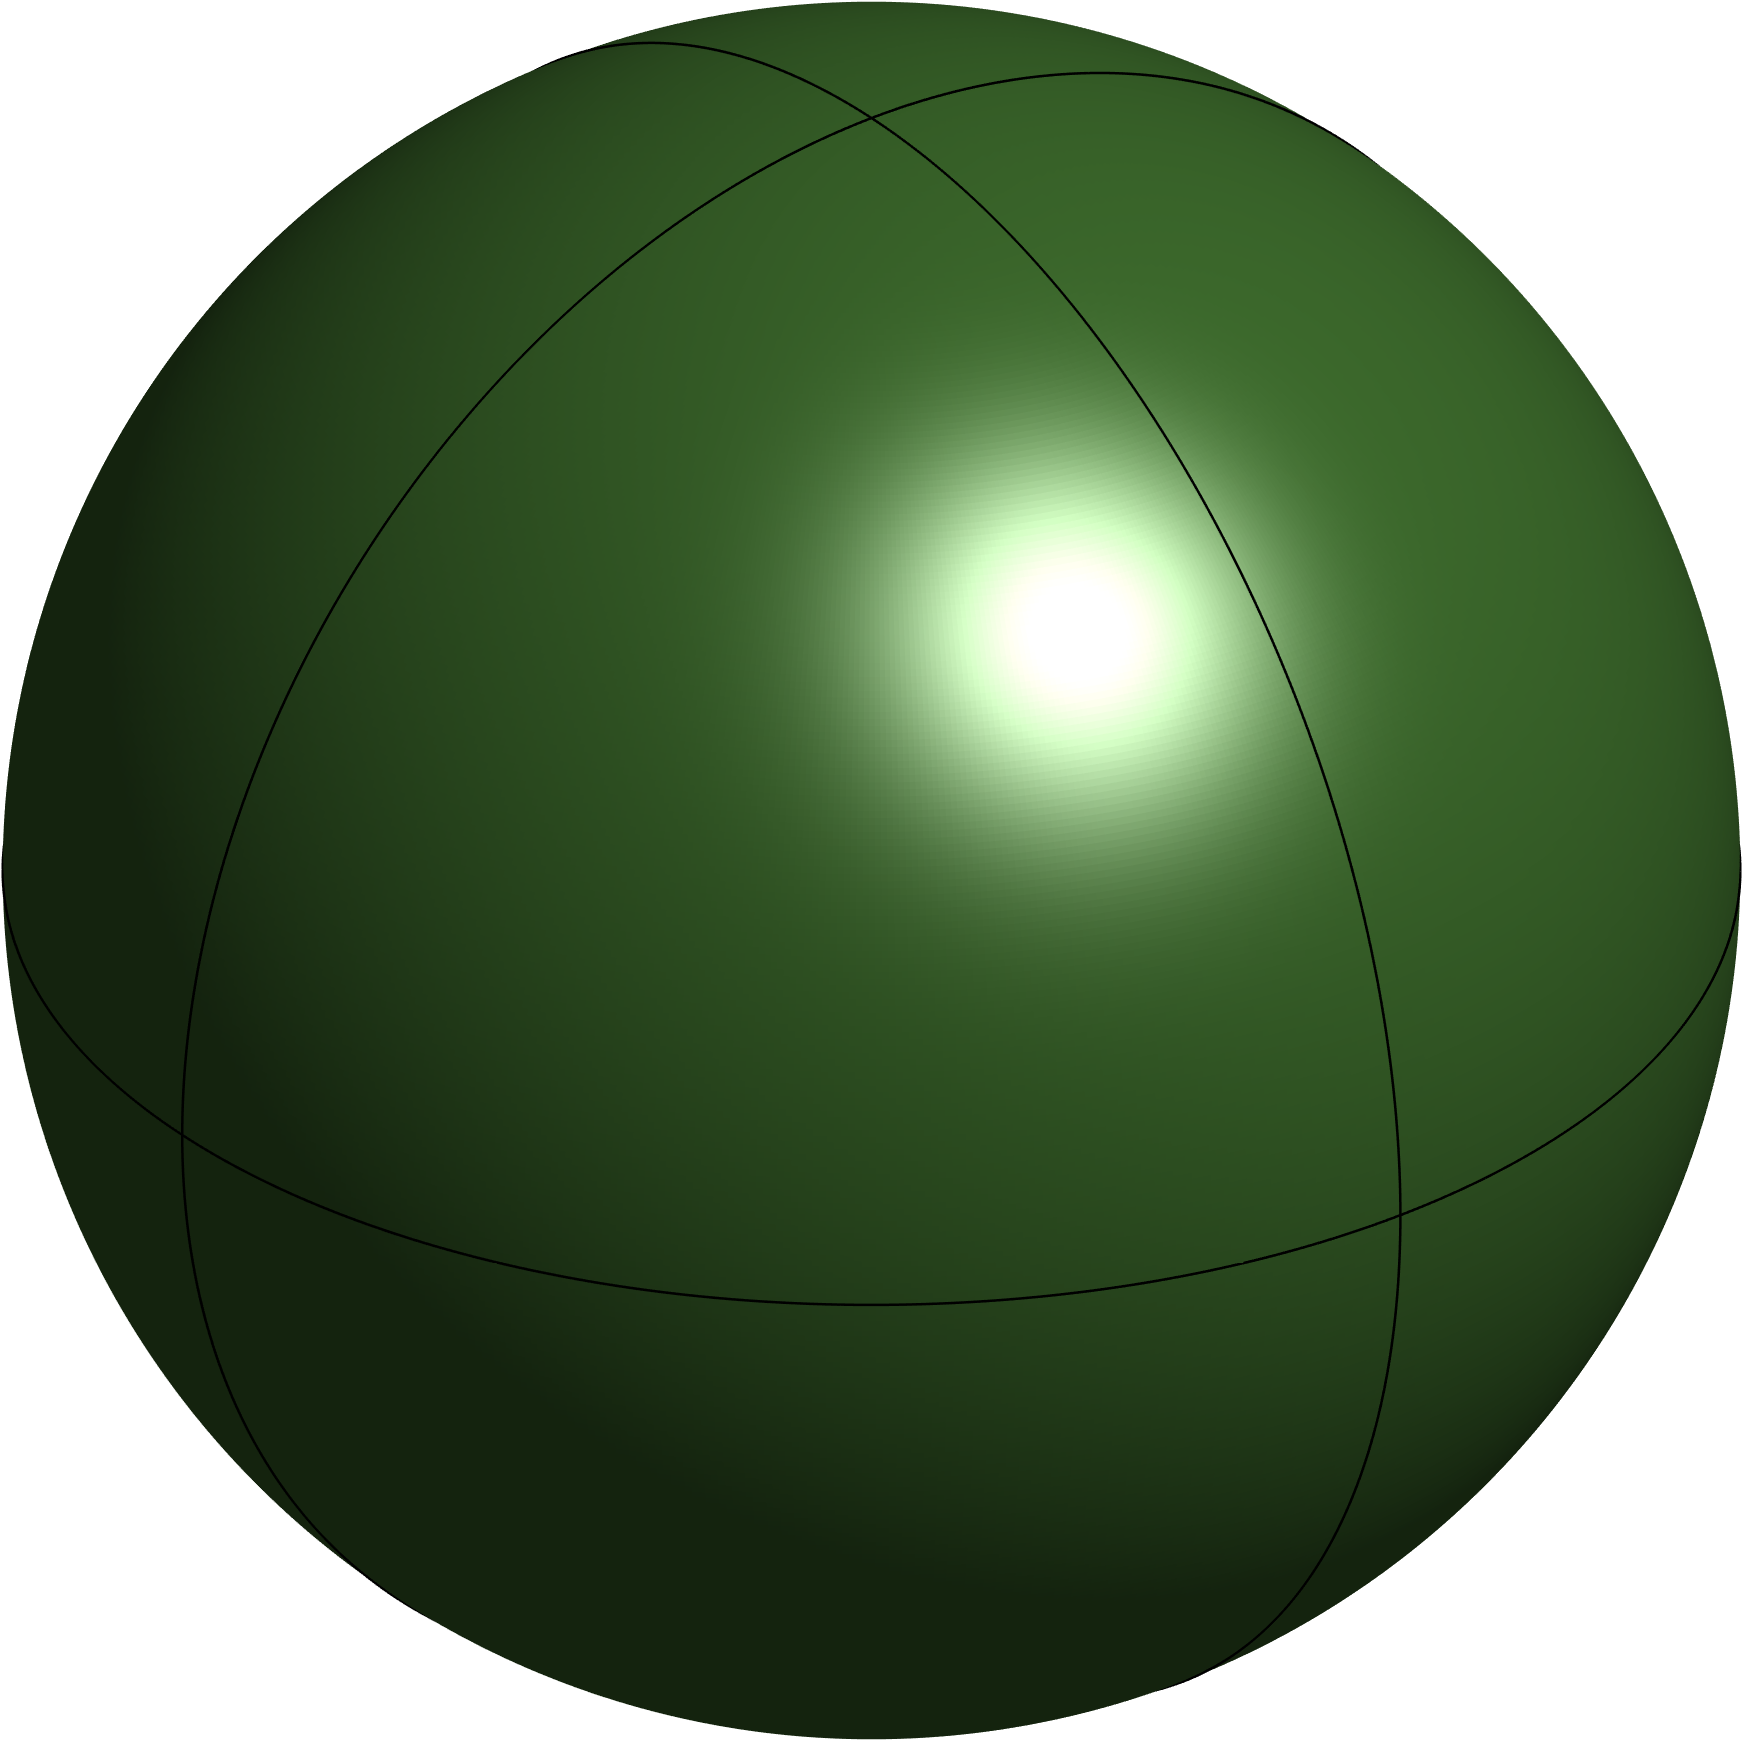
\includegraphics[width=0.3\textwidth]{../../graphics/sphericalShell/sphericalShellMesh1_2_0}
%	\includegraphics[width=0.3\textwidth]{\graphicsFolder/Figure2a}
	~
	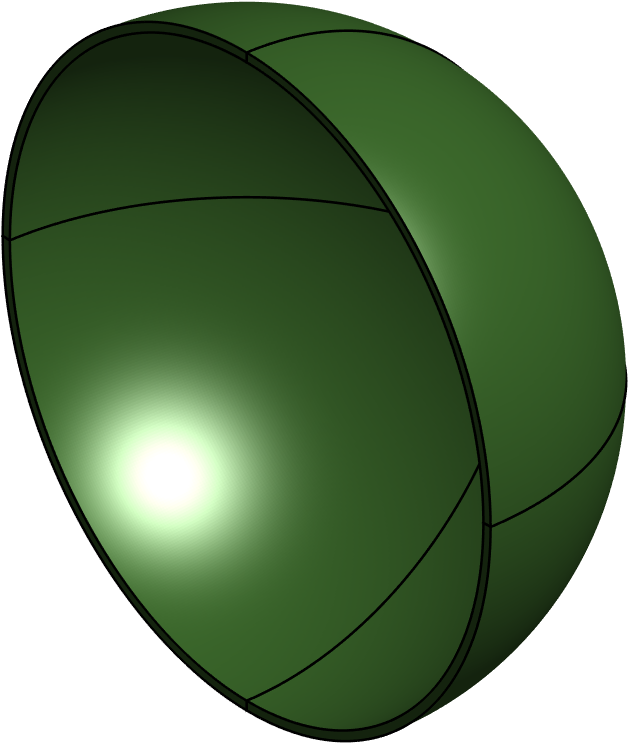
\includegraphics[width=0.25\textwidth]{../../graphics/sphericalShell/halfSphericalShellMesh}
%	\includegraphics[width=0.25\textwidth]{\graphicsFolder/Figure2b}
	\caption[Exact geometry of a spherical shell using 8 elements]{Exact geometry of a spherical shell using 8 elements.}
	\label{Fig2:SphericalShell}
\end{figure}

It has been shown that the continuity of the basis functions plays an important role for the accuracy of solving elliptical problems (for instance the Helmholtz equation), see~\cite{BeiraodaVeiga2011sef} and~\cite{BeiraodaVeiga2014mao}. This motivates the use of IGA even further, as IGA enables control of the continuity of the basis function up to $C^{p-1}$ (in contrast with the $C^0$-continuity restriction in FEA). IGA has proven to be promising in a host of areas related to the problem at hand, which yields further motivation in the use of IGA. For instance, in~\cite{nortoft2015iao} the method was shown to be suited for the more complex scenario of sound propagation through laminar flow.

In addition to IGA, the so-called infinite element method (IEM) has been chosen to handle the boundary conditions at the artificial boundary. Typically, the boundary element method (BEM) \cite{Sauter2011bem,Schanz2007bea} has been used for this purpose. However, for higher frequencies and complex geometries, BEM becomes computationally expensive (although improvement in performance has been done in the recent decades \cite{Liu2012raa}). The main motivation for the infinite element method is computational efficiency as reported by Burnett~\cite{Burnett1994atd} and Gerdes and Demkowicz~\cite{Gerdes1996so3}.

Before starting on the full ASI problem, it is important to establish good results for the IEM. This method only applies for the outer fluid, and it would thus be natural to first investigate the scattering problem on rigid objects (that is, no acoustic-structure interaction occurs). An introduction to the IEM is presented in \Cref{Sec2:exteriorHelmholtz}. The extension to ASI problems (presented in~\Cref{Sec2:coupledFluidStruct}) naturally follows from the implementation of rigid scattering using IEM. In \Cref{Sec2:resultsDisc} the results obtained for both rigid and elastic scattering on a spherical shell is presented. Results for rigid scattering from a mock shell are included to investigate condition numbers. Moreover, results for a simplified submarine is presented to illustrate the performance of the implementation on complex geometries. Finally, conclusions and suggested future work can be found in \Cref{Sec2:conclusions}. 